\chapter{Null geodesics and images in Kerr spacetime}
\label{s:gik}

\minitoc

\section{Introduction}

Having investigated the properties of generic causal geodesics
in Schwarzschild spacetime in Chap.~\ref{s:ges}, we focus here on null
geodesics.


\section{Main properties of null geodesics} \label{s:gik:properties}

We shall distinguish the null geodesics with $E=0$ (the so-called \emph{zero-energy} geodesics,
cf. Sec.~\ref{s:gek:sign_E})
 from those having
$E \neq 0$. Indeed, in the latter case, we will rescale the angular momentum
$L$ and the Carter constant $Q$ by $E$, so that only two constants of motion become
pertinent for the study: $L/E$ and $Q/E^2$.
We thus treat first the particular case $E=0$.

\subsection{Null geodesics with $E=0$}


First, we note that a geodesic $\Li$ with $E=0$ cannot exist outside the ergoregion
$\mathscr{G}$, by virtue of the result (\ref{e:gek:E_positive}). In particular,
it cannot exist far from the black hole.

Another property of null geodesics with $E=0$ is to have a nonnegative Carter constant:
\be \label{e:gik:Q_nonneg_E_zero}
   \encadre{ Q \geq 0 }_{E=0} .
\ee
This follows immediately from the result of Sec.~\ref{s:gek:th_motion}
stating that a necessary condition for $Q < 0$ is $a\neq 0$ and
$|E| > \sqrt{\mu^2 + L^2/a^2}$. Specializing this last inequality to $\mu=0$
and $E=0$, we get $0 > |L|$, which is impossible.

Besides, if $\Li$ has some part in $\M_{\rm I}$ (necessarily in the outer ergoregion)
or in $\M_{\rm III}$ (necessarily in the inner ergoregion),
the constraint (\ref{e:gek:future_directed_Carter})
reduces to $L<0$:
\be \label{e:gik:E_zero_L_neg_ergo}
    \Li \cap (\M_{\rm I} \cup \M_{\rm III}) \neq  \varnothing \quad \Longrightarrow \quad L < 0 .
\ee
We shall see below that actually $L \leq 0$ for all zero-energy null geodesics, as soon as $a\neq 0$.

The equations of geodesic motion expressed in terms of the Mino parameter $\lambda'$
[system (\ref{e:gek:eom_Mino})] simplify considerably for a geodesic $\Li$ with $\mu=0$ and $E=0$:
\begin{subequations}
\begin{align}
&  \derd{t}{\lambda'} = - \frac{2 a m L r}{\Delta} \label{e:gik:eom_t_E_zero} \\
&  \derd{r}{\lambda'} = \eps_r \sqrt{ R(r) }  \label{e:gik:eom_r_E_zero}\\
&  \derd{\th}{\lambda'} = \eps_\th \sqrt{\Theta(\th)}  \\
&  \derd{\ph}{\lambda'}  = \frac{L}{\Delta\sin^2\th} \left( r^2 - 2 m r + a^2\cos^2\th \right) ,
                                \label{e:gik:eom_ph_E_zero}
\end{align}
\end{subequations}
with [cf. Eqs.~(\ref{e:gek:R_r_powers}) and (\ref{e:gek:Theta_Q})]:
\be \label{e:gik:R_E_zero}
    R(r) = - (Q+L^2) r^2 + 2m (Q+L^2) r - a^2 Q
\ee
\be \label{e:gik:Theta_E_zero}
    \Theta(\th) = Q - \frac{L^2}{\tan^2\th} .
\ee
By combining (\ref{e:gik:eom_t_E_zero}) and (\ref{e:gik:eom_ph_E_zero}), we get
\be
    \encadre{ \left. \derd{\ph}{t} \right| _{\Li} = \frac{2mr - r^2 - a^2\cos^2\th}{2 a m r\sin^2\th} }_{E=0} .
\ee
It is remarkable that this expression does not depend on $L$ or $Q$; it is therefore the
same for all zero-energy null geodesics. Moreover, we note that the numerator
of the right-hand side is always positive or zero in the closure $\overline{\mathscr{G}}$ of the ergoregion,
which is precisely defined by $2mr - r^2 - a^2\cos^2\th \geq 0$ (cf. Sec.~\ref{s:ker:ergoregion})
and where $\Li$ is necessarily confined. Since moreover $r > 0$ in $\overline{\mathscr{G}}$,
we conclude that
\be
    \left. \derd{\ph}{t} \right| _{\Li} \geq 0 .
\ee


To proceed, we shall distinguish the subcases $Q\neq 0$ and $Q=0$.

\subsubsection{Case $Q\neq 0$}

This case actually corresponds to $Q > 0$, since $Q<0$ is forbidden by
(\ref{e:gik:Q_nonneg_E_zero}). We set
\be \label{e:gik:def_L_bar}
    \bar{L} := \frac{L}{\sqrt{Q}}
\ee
and rewrite expression (\ref{e:gik:R_E_zero}) for $R(r)$ as
\be \label{e:gik:R_E_zero_Lb}
    R(r)/Q  = - (1 + \bar{L}^2) r^2 + 2m (1 + \bar{L}^2) r - a^2 .
\ee
Since $1 + \bar{L}^2 \neq 0$, this is a second-order polynomial in $r$,
the two roots of which are
\be \label{e:gik:E_zero_rmin_rmax}
    r_{\rm min} = m - \sqrt{m^2 - \frac{a^2}{1 + \bar{L}^2}}
    \qand
    r_{\rm max} = m + \sqrt{m^2 - \frac{a^2}{1 + \bar{L}^2}} .
\ee
Since $m^2 \geq a^2$, the two roots are real. They are distinct
except for $a=m$ and $L=0$.
The range of radial motion being determined by $R(r)\geq 0$
[Eq.~(\ref{e:gek:R_non_neg})], we get
\be
    r_{\rm min} \leq r \leq r_{\rm max} ,
\ee
with a turning point at $r_{\rm min}$ and at $r_{\rm max}$.
Given that $r_- = m - \sqrt{m^2 - a^2}$ and $r_+ = m + \sqrt{m^2 - a^2}$
[Eq.~(\ref{e:ker:def_r_pm})], we note that
\be
     0 \leq r_{\rm min} \leq r_- \leq m \leq r_+ \leq r_{\rm max} \leq 2 m ,
\ee
with $r_{\rm min} = 0$ for $a = 0$ or $\bar{L}^2 \to +\infty$,
$r_{\rm min} = r_-$ for $L=0$, $r_{\rm max} = 2m$ for $a=0$
or $\bar{L}^2 \to +\infty$ and $r_{\rm max} = r_+$ for $L=0$.
If $L\neq 0$ and $a\neq 0$, then $r_{\rm max} > r_+$, so that $\Li$ has a part in the outer
ergoregion and (\ref{e:gik:E_zero_L_neg_ergo}) implies that $L < 0$. Hence
\be \label{e:gik:E_zero_Qnz_L_neg}
    a\neq 0 \implies L \leq 0 .
\ee

Let us consider a zero-energy null geodesic $\Li$ emitted outward (i.e.
with $\epsilon_r = +1$) from a point $A$ in the outer ergoregion $\mathscr{G}^+$.
The coordinate $r$ increases along $\Li$ from $r_A$ to $r_{\rm max}$, which
corresponds to a $r$-turning point. Then $r$ decreases to $r_+$, which means
that $\Li$
crosses the black hole event horizon $\Hor$ and enters the region $\M_{\rm II}$.
In all $\M_{\rm II}$, $r$ keeps decreasing and reaches $r_-$. There $\Li$
crosses the inner horizon $\Hor_{\rm in}$ and enters the region $\M_{\rm III}$,
where $r$ continues to decrease until it reaches $r_{\rm min}$. The latter
corresponding to a $r$-turning point, $r$ starts to increase and reaches
$r_-$ again. There one might think that $\Li$ crosses the inner horizon
$\Hor_{\rm in}$ and enters into $\M_{\rm II}$. But this is impossible since
$\Hor_{\rm in}$ is a 1-way membrane: it can be crossed by a causal curve
from $\M_{\rm II}$ to $\M_{\rm III}$ but not in the reverse way. Moreover, $r$
could not continue to increase into $\M_{\rm II}$ since $r$ must be decreasing
towards the future in all this region (this follows from the hypersurfaces
$r=\mathrm{const}$ being spacelike in $\M_{\rm II}$, cf. Sec.~\ref{s:ker:Killing_hor}).
The solution to this apparent puzzle is immediate as soon as one realizes
that the boundary $r = r_-$ of $\M_{\rm III}$ is not entirely constituted
by $\Hor_{\rm in}$: it also comprises a null hypersurface that separates
$\M_{\rm III}$ from a region distinct from $\M_{\rm II}$ in
the maximally extended Kerr spacetime, cf. Fig.~\ref{f:ker:max_ext}. This region
is a ``time-reversed'' copy of $\M_{\rm II}$ and is
denoted by ${\M_{\rm II}^*}'$ in Fig.~\ref{f:ker:max_ext} (cf. Sec.~\ref{s:ker:max_extension}
for details).
So actually, when it reaches $r=r_-$, the null geodesic $\Li$ enters
${\M_{\rm II}^*}'$. There $r$ necessarily increases towards the future, at
the opposite of $\M_{\rm II}$. It reaches then $r=r_+$, where $\Li$
crosses a white hole\index{white hole} horizon and emerges into
the asympototically flat region $\M_{\rm I}''$, as illustrated in
Fig.~\ref{f:gik:zero_ener_traj}. The region $\M_{\rm I}''$ is similar
to $\M_{\rm I}$. In particular, $\Li$ is confined into the outer ergoregion
of $\M_{\rm I}''$, having a $r$-turning point at $r=r_{\rm max}$ (same value
(\ref{e:gik:E_zero_rmin_rmax}) as in $\M_{\rm I}$). Then a new cycle
begins, with $\Li$ entering the future event horizon of $\M_{\rm I}''$.

\begin{figure}
\centerline{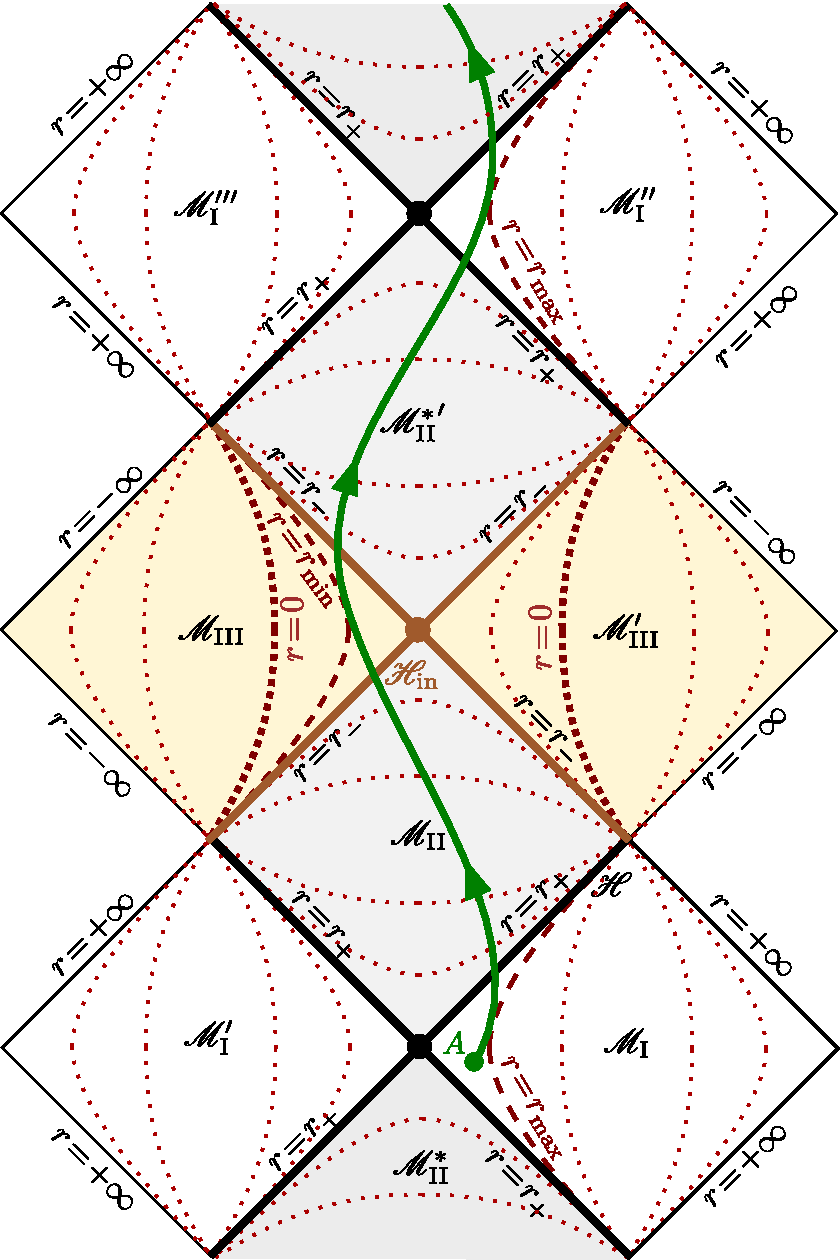
\includegraphics[width=0.6\textwidth]{gik_zero_ener_traj.pdf}}
\caption[]{\label{f:gik:zero_ener_traj} \footnotesize
Trajectory in the extended Kerr spacetime of a null geodesic
with $E=0$, $Q>0$ and $L<0$, emitted from a point $A$ in the outer ergoregion.
}
\end{figure}

The $\theta$-motion of $\Li$ is constrained by $\Theta(\th) \geq 0$ [Eq.~(\ref{e:gek:Theta_non_neg})],
which, given expression~(\ref{e:gik:Theta_E_zero}) for $\Theta$, is
equivalent to
\be
    \th_{\rm min} \leq \th \leq \pi - \th_{\rm min} \quad\mbox{with}\quad
    \th_{\rm min} := \arctan (-\bar{L}) .
\ee
For $L = 0$, one has $\th_{\rm min} = 0$, so that $\th$ takes all values in the
range $[0,\pi]$, which means that $\Li$
crosses repeatedly the rotation axis. For $L< 0$, one has $0 < \th_{\rm min} < \pi/2$ and
$\Li$ oscillates symmetrically about the equatorial plane,
having two $\th$-turning points, at $\th_{\rm min} $ and $\pi-\th_{\rm min}$. Of course, we
recover the general results for $Q>0$ of Sec.~\ref{s:gek:th_motion}.

We can obtain $r$ as a function of $\th$ along $\Li$ by evaluating the integrals
in the identity (\ref{e:gek:integr_Mino}):
\[
    \dashint_{r_0}^r \frac{\eps_r \, \D \bar{r}}{\sqrt{R(\bar{r})}}
   = \dashint_{\th_0}^\th \frac{\eps_\th \, \D \bar{\th}}{\sqrt{\Theta(\bar{\th})}}
\]
Using (\ref{e:gik:R_E_zero_Lb}) and (\ref{e:gik:Theta_E_zero}), we get on
any portion of $\Li$ where $\eps_r$ and $\eps_\th$ are constant,
\[
    \eps_r \int_{r_0}^r
    \frac{\D \bar{r}}{\sqrt{- (1 + \bar{L}^2) \bar{r}^2 + 2m (1 + \bar{L}^2) \bar{r} - a^2}}
    = \eps_\th \int_{\th_0}^\th \frac{\D \bar{\th}}{\sqrt{1 - \bar{L}^2/\tan^2\bar{\th}}} .
\]
The changes of variables
\[
    x = \frac{r/m - 1}{\sqrt{1 - \frac{a^2}{m^2(1 + \bar{L}^2)}}}
    \qand
    \mu = \cos\th
\]
lead to
\[
   \frac{\eps_r}{\sqrt{1 + \bar{L}^2}} \int_{x_0}^x \frac{\D\bar{x}}{\sqrt{1 - \bar{x}^2}}
   = - \eps_\th \int_{\cos\th_0}^{\cos\th} \frac{\D\mu}{\sqrt{1 - (1 + \bar{L}^2)\mu^2}} .
\]
The integration is then immediate:
$\arcsin x = - \eps_r \eps_\th \arcsin(\sqrt{1 + \bar{L}^2} \cos\th) + K$,
where $K$ is a constant, from which we get
\be \label{e:gik:E_zero_r_theta}
   \encadre{ r = m + m\sqrt{1 - \frac{a^2}{m^2(1 + \bar{L}^2)}} \; \sin \left[
        K - \eps_r \eps_\th \arcsin\left(\sqrt{1 + \bar{L}^2} \cos\th\right) \right] }.
\ee
Since $\sqrt{1 + \bar{L}^2} \cos\th_{\rm min} = 1$, we see that the constant
$K$ is related to the value of $r$ at $\th = \th_{\rm min}$ by
\be \label{e:gik:E_zero_K}
    K =  \arcsin \left( \frac{r(\th_{\rm min})/m - 1}{\sqrt{1 - \frac{a^2}{m^2(1 + \bar{L}^2)}}} \right)
    + \eps_r \eps_\th \frac{\pi}{2} .
\ee
Note that $K$ is not a constant all along $\Li$, but only on portions where
$\eps_r$ and $\eps_\th$ are constant.
Expression~\ref{e:gik:E_zero_r_theta} gives the trace of the zero-energy
null geodesic $\Li$ in a meridional plane. It depends on $Q$ and $L$ only
through the ratio $\bar{L} := L / \sqrt{Q}$. It depends as well on the value of
$r$ at $\th_{\rm min}$ via $K$, as it appears in Eq.~(\ref{e:gik:E_zero_K}).
An example is shown in Fig.~\ref{f:gik:zero_ener_merid} for $a/m = 0.9$, $L / \sqrt{Q} = -1$
and $r(\th_{\rm min}) = 1.5\, m$. It has $\th_{\rm min} = \pi/4$,
$r_{\rm min} \simeq 0.229\, m$ and $r_{\rm max} \simeq 1.771\, m$,
while for $a/m = 0.9$, one has $r_- \simeq 0.564\, m$ and $r_+ \simeq 1.436\, m$.
For concreteness, the arrows indicate some direction of motion, but depending upon some
initial conditions, the opposite direction is possible.
In particular, one may consider that the geodesic is the same as that shown
in Fig.~\ref{f:gik:zero_ener_traj}, being emitted outward in the outer ergoregion
from a point $A$ in the equatorial plane ($\th=\pi/2$).

\begin{figure}
\centerline{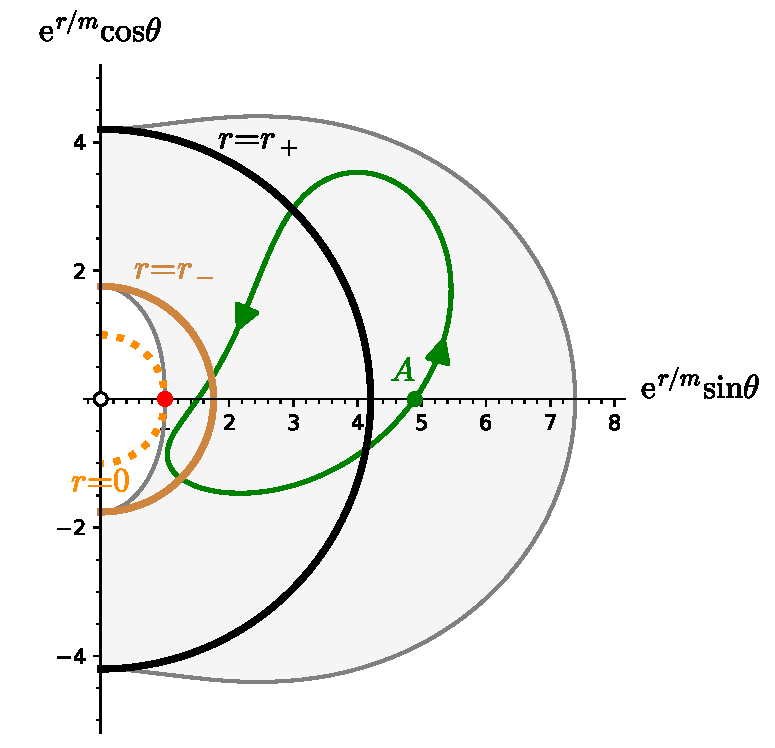
\includegraphics[width=0.6\textwidth]{gik_zero_ener_merid.pdf}}
\caption[]{\label{f:gik:zero_ener_merid} \footnotesize
Trajectory in the meridional plane, as given by Eq.~(\ref{e:gik:E_zero_r_theta}), of a null geodesic (green curve)
with $E=0$, $Q>0$, $L = - \sqrt{Q}$ and $r(\th_{\rm min}) = 1.5 \, m$
in the Kerr spacetime with $a/m = 0.9$.
The meridional plane is described in terms of
O'Neill exponential coordinates $x = \mathrm{e}^{r/m}\sin\th$ and $z = \mathrm{e}^{r/m}\cos\th$,
as in Figs.~\ref{f:ker:ergo_a90} -- \ref{f:ker:ergo_a99}.
The ergoregion is shown in grey.
The black (resp. blight rown) half-circle at $r=r_+$ (resp. $r=r_-$)
is the trace of the outer (resp. inner) Killing horizon.
The dotted orange half-circle marks the locus of $r=0$, with the
red dot indicating the curvature singularity at $r=0$ and $\th=\pi/2$.
The area $r> r_+$
corresponds to the regions $\M_{\rm I}$ and $\M_{\rm I}''$ in Fig.~\ref{f:gik:zero_ener_traj},
the area  $r_- < r < r_+$
corresponds to the regions $\M_{\rm II}$ and ${\M_{\rm II}^*}'$  in Fig.~\ref{f:gik:zero_ener_traj} and the area $r < r_-$
corresponds to the region $\M_{\rm III}$ in Fig.~\ref{f:gik:zero_ener_traj}.
\textsl{[Figure generated by the notebook \ref{s:sam:Kerr_null_geod_zero_ener}]}
}
\end{figure}

\subsubsection{Case $Q=0$}

If the zero-energy null geodesic $\Li$ has a vanishing Carter constant $Q$, Eq.~(\ref{e:gik:Theta_E_zero}) reduces to $\Theta(\th) = -L^2 / \tan^2\th$,
so that the constraint $\Theta(\th) \geq 0$ [Eq.~(\ref{e:gek:Theta_non_neg})]
implies $L=0$ or $\th = \pi/2$ .

In the first case, the four constants of motion $\mu$, $E$, $L$ and $Q$ are
zero. By virtue of the result (\ref{e:gek:all_const_zero}), $\Li$
is nothing but a null geodesic generator of the event horizon $\Hor$ or of the
inner horizon $\Hor_{\rm in}$.

In the second case ($\th=\pi/2$), $\Li$ is confined to the equatorial plane.
If $L=0$, we are back to the first case: $\Li$ is null geodesic generator of $\Hor$ or
$\Hor_{\rm in}$ lying in the equatorial plane.
If $L\neq 0$, the radial motion of $\Li$ is governed by Eq.~(\ref{e:gik:eom_r_E_zero}) with the
expression (\ref{e:gik:R_E_zero}) of $R(r)$ reduced to
\be
    R(r) = L^2 r (2m - r) .
\ee
The constraint $R(r) \geq 0$ [Eq.~(\ref{e:gek:R_non_neg})] implies then
that the motion is within the range $0 \leq r \leq 2 m$, with $r=2m$
being a $r$-turning point, since it is a simple root of $R(r)$ (cf. Sec.~\ref{s:gek:turning_points}).
It corresponds to the outer edge of the ergoregion in the equatorial plane,
cf. Eq.~(\ref{e:ker:r_ergo_p_eq}). Hence we have necessarily $\Li\cap \M_{\rm I} \neq \varnothing$
and (\ref{e:gik:E_zero_L_neg_ergo}) applies: $L < 0$.
The inner boundary of the radial motion, $r=0$, is the ring singularity.
Accordingly, in the maximally extended Kerr spacetime, $\Li$ starts at the ring
singularity in a $\M_{\rm III}$-type region (cf. Fig.~\ref{f:gik:zero_ener_traj_q0}),
has $r$ increasing, enters
a $\M_{\rm II}^*$-type region (time reversed copy of $\M_{\rm II}$), emerges
in $\M_{\rm I}$ via the white hole horizon at $r=r_+$ and reaches a $r$-turning point at
$r=2m$, then $r$ decreases continuously until $\Li$ terminates at the ring
singularity of $\M_{\rm III}$, after having crossed the black hole horizon $\Hor$
and the inner horizon $\Hor_{\rm in}$.
This trajectory, depicted in
Fig.~\ref{f:gik:zero_ener_traj_q0}, is similar to that for $Q\neq 0$
shown in Fig.~\ref{f:gik:zero_ener_traj}, except that it is ``blocked''
by two ring singularities and cannot oscillate foreover between distinct
$\M_{\rm I}$-type regions.

\begin{figure}
\centerline{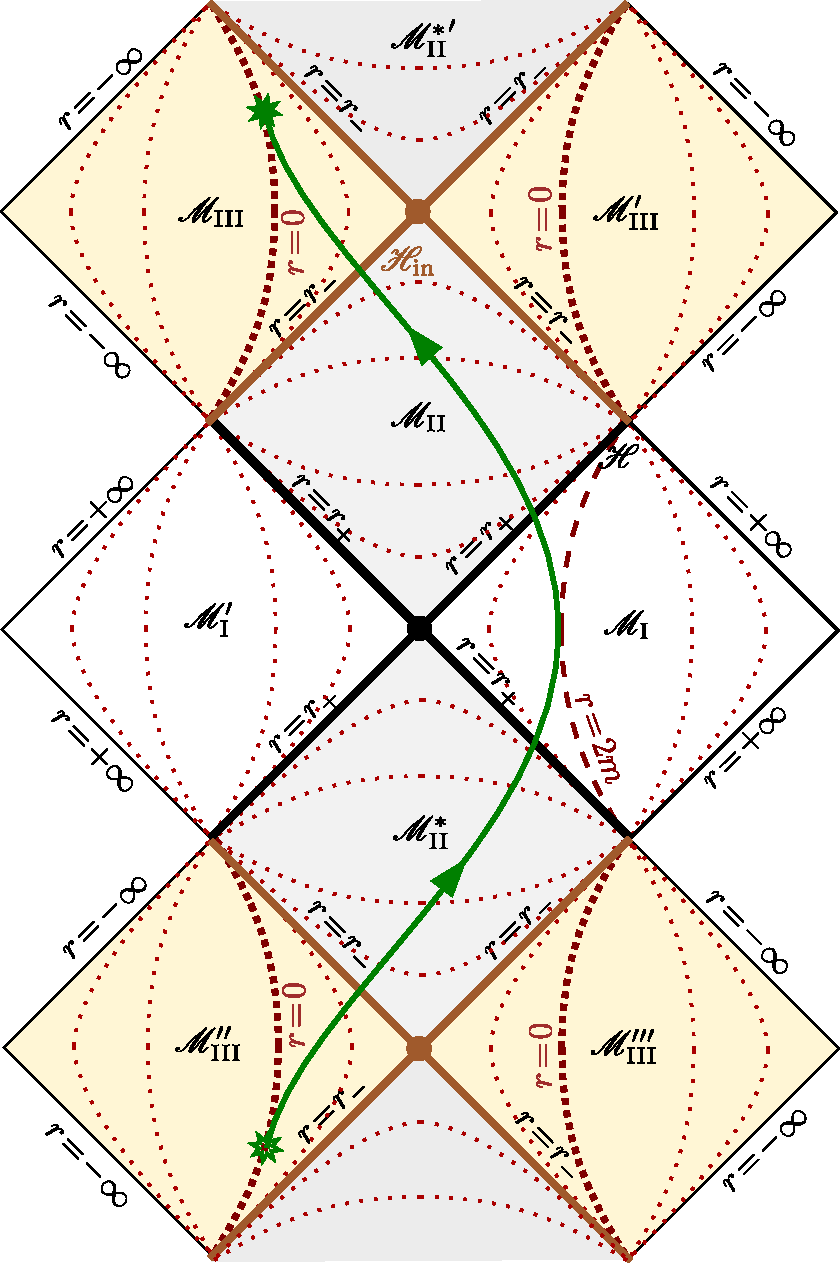
\includegraphics[width=0.6\textwidth]{gik_zero_ener_traj_q0.pdf}}
\caption[]{\label{f:gik:zero_ener_traj_q0} \footnotesize
Trajectory in the extended Kerr spacetime of a null geodesic
with $E=0$, $Q=0$ and $L<0$.
}
\end{figure}


\begin{remark}
For $Q\neq 0$ and $L\neq 0$, the limit $Q\to 0$ corresponds to
$\bar{L}^2 \to +\infty$ [cf. Eq.~(\ref{e:gik:def_L_bar})], so that
Eq.~(\ref{e:gik:E_zero_rmin_rmax}) yields
$r_{\rm min}\to 0$ and $r_{\rm max}\to 2m$.
We recover then the range $[0, 2m]$ for $r$ obtained here for $Q=0$.
\end{remark}


We conclude that
\begin{greybox}
Any null geodesic with $E=0$ and $Q=0$
is either a null generator of one of the two Killing horizons
$\Hor$ or $\Hor_{\rm in}$ (in which case, it has $L=0$) or it has
$L < 0$, lies in the equatorial plane,
emanates from a ring singularity, reaches the outer ergosphere ($r=2m$),
where it has a $r$-turning point, and terminates at a ring singularity.
\end{greybox}

Regarding the sign of $L$, we can combine the above result with that
obtained for $Q\neq 0$ [Eq.~(\ref{e:gik:E_zero_Qnz_L_neg})] to conclude:
\begin{greybox}
For $a\neq 0$, any null geodesic with $E=0$ has necessarily
\be
    \encadre{ L \leq 0 }_{{a\neq 0\atop E=0}}.
\ee
\end{greybox}



\subsection{Equations of geodesic motion for $E\neq 0$}

When $E\neq 0$, we introduce the reduced constants of motion
\be
    \encadre{\ell := \frac{L}{E}} \qand
    \encadre{q := \frac{Q}{E^2}} .
\ee
Note that, in geometrized units ($G=1$ and $c=1$), $\ell$ has the dimension of
a length and $q$ that of a squared length.

The nonnegative property of Carter constant $\mathscr{K}$ [Eq.~(\ref{e:ges:K_non_negative})],
along with the identity (\ref{e:gek:def_Q}) leads to the following constraint on
the parameters $\ell$ and $q$:
\be \label{e:gik:q_ell_a_constraint}
    \encadre{ q + (\ell - a)^2 \geq 0} .
\ee

\begin{example}[Principal null geodesic]
A principal null geodesic has $E\neq 0$ if, and only if, it does not belong to the outgoing
family generating the horizon $\Hor$ or $\Hor_{\rm in}$. This follows immediately from
Eqs.~(\ref{e:gek:ingoing_null_E_L}) and (\ref{e:gek:outgoing_null_E_L}).
One has then
$L = a E\sin^2\th_0$
[Eqs.~(\ref{e:gek:ingoing_null_E_L}) and (\ref{e:gek:outgoing_null_E_L})]
and $Q = - a^2 E^2 \cos^2\th_0$ [Eq.~(\ref{e:gek:Q_principal_null})], where
$\th_0$ is the constant value of $\th$ along the geodesic. We have thus
\be \label{e:gik:principal_null_l_q}
    \ell = a \sin^2\th_0 \qand q = - a^2 \cos^4\th_0 .
\ee
This yields
\be
    q + (\ell - a)^2  = 0 ,
\ee
so that (\ref{e:gik:q_ell_a_constraint}) is saturated for principal null
geodesics.
\end{example}

The equations of motion in term of the Mino parameter $\lambda'$,
Eqs.~(\ref{e:gek:eom_Mino}) specialized to $\mu=0$, can be rewritten as
\begin{subequations}
\label{e:gik:eom_Mino}
\begin{align}
& \encadre{ \frac{1}{E} \derd{t}{\lambda'} = \frac{r^2 + a^2}{\Delta} (r^2 + a^2 - a \ell) + a ( \ell - a \sin^2\th ) } \label{e:gik:dtdl_Mino} \\
& \encadre{ \frac{1}{E} \derd{r}{\lambda'} = \eps_r \sqrt{ \mathcal{R}(r) } } \label{e:gik:drdl_Mino}\\
& \encadre{ \frac{1}{E} \derd{\th}{\lambda'} = \eps_\th \sqrt{\tilde\Theta(\th)} } \label{e:gik:dthdl_Mino}\\
& \encadre{ \frac{1}{E} \derd{\ph}{\lambda'}  = \frac{\ell}{\sin^2\th}
    + \frac{a}{\Delta}(2m r - a \ell) } , \label{e:gik:dphdl_Mino}
\end{align}
\end{subequations}
with
\be
    \mathcal{R}(r) := \frac{R(r)}{E^2}
    \qand
    \tilde\Theta(\th) := \frac{\Theta(\th)}{E^2} .
\ee
From the general expressions (\ref{e:gek:def_R_Q}), (\ref{e:gek:R_r_powers}) and (\ref{e:gek:Theta_Q}) specialized to $\mu=0$, we get
\begin{subequations}
\label{e:gik:mcR}
\begin{align}
    &\encadre{\mathcal{R}(r) = (r^2 + a^2 - a \ell)^2 - \Delta \left[ q + (\ell -a)^2 \right] }
      \label{e:gik:mcR_Delta}\\
    &\encadre{\mathcal{R}(r) =  r^4 + (a^2 - \ell^2 - q) r^2 + 2m\left[ q + (\ell -a)^2 \right] r
    - a^2 q } \label{e:gik:mcR_powers}
\end{align}
\end{subequations}
and
\be \label{e:gik:tTheta}
    \encadre{ \tilde\Theta(\th) = q + \cos^2\th \left( a^2
    - \frac{\ell^2}{\sin^2\th} \right) } .
\ee

It suffices to use the parameter $\lambda'' := |E| \lambda'$ to make $E$
disappear from the system~(\ref{e:gik:eom_Mino}). We therefore conclude that
\begin{greybox}
In Kerr spacetime, a null geodesic with $E\neq 0$  is entirely determined
by the two constants $(\ell,q)$ and by the values of the two signs $\eps_r=\pm 1$ and $\eps_\th=\pm 1$
at a given point.
\end{greybox}

\begin{example}[Principal null geodesic]
Given the values (\ref{e:gik:principal_null_l_q}) of $\ell$ and $q$
for a principal null geodesic, Eq.~(\ref{e:gik:mcR_powers}) reduces to
a simple expression for the quartic polynomial $\mathcal{R}$:
\be \label{e:gik:mR_PNG}
    \mathcal{R}(r) = \left( r^2 + a^2 \cos^2 \th_0 \right)^2 .
\ee
We note that $\mathcal{R}(r) = \rho^4$, which makes sense because $\th = \th_0$
is constant along such a geodesic. For any principal null geodesics lying
in the equatorial plane, the polynomial simplifies even further:
\be
    \mathcal{R}(r) = r^4, \qquad \left(\th_0 = \frac{\pi}{2} \right) .
\ee
\end{example}

\begin{figure}
\centerline{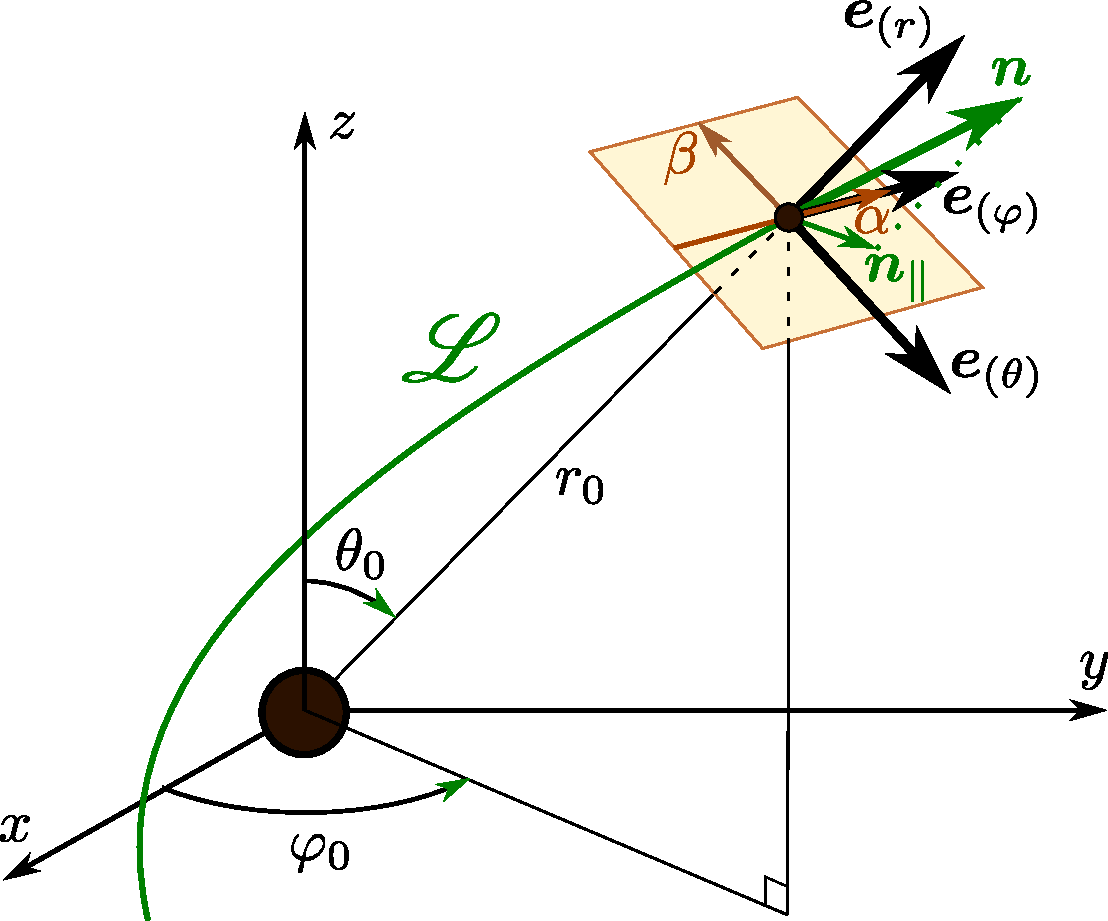
\includegraphics[width=0.6\textwidth]{gik_obs_screen.pdf}}
\caption[]{\label{f:gik:obs_screen} \footnotesize
Impact of a null geodesic $\Li$ onto the screen of a remote observer. $(x,y,z)$ are the Cartesian Boyer-Lindquist coordinates
defined by Eq.~(\ref{e:gek:Cartesian_BL}).
}
\end{figure}

\subsubsection{Remote observer's screen}

The constants $(\ell,q)$ are closely related to the impact coordinates $(\alpha,\beta)$
on the screen of an asymptotic inertial observer (cf. Sec.~\ref{s:ker:asymp_inertial_obs})
in case the null geodesic $\Li$ reaches the asymptotic region $r\to +\infty$.
Indeed let us consider an asymptotic inertial observer $\Obs$ located at (fixed) Boyer-Lindquist
coordinates $(r_0, \th_0, \ph_0)$, with $r_0 \gg m$ (cf. Fig.~\ref{f:gik:obs_screen}).
The orthonormal frame of $\Obs$ is $\w{e}_{(0)} =\w{\xi}$, $\w{e}_{(r)} = \wpar_r$,
$\w{e}_{(\th)} = r_0^{-1} \wpar_\th$ and $\w{e}_{(\ph)} = (r_0\sin\th_0)^{-1} \wpar_\ph$
[Eq.~(\ref{e:ker:def_ZAMO_frame}) with $r = r_0\to +\infty$].
Let us assume that the observer set up a screen (via a telescope) centered on the direction to the
black hole, i.e. such that $\w{e}_{(r)}$ is the normal to the screen. The 4-momentum of the photon
having $\Li$ as worldline at the location of $\Obs$ writes
\[
    \w{p} = p^t \, \w{\xi} + p^r \, \w{e}_{(r)} + p^\th r_0 \, \w{e}_{(\th)}
    + p^\ph r_0 \sin\th_0 \, \w{e}_{(\ph)} =  E (\w{\xi} + \w{n}) ,
\]
where the second equality follows from the orthogonal decomposition (\ref{e:fra:p_E_V}) with respect to
$\Obs$, $\w{\xi}$ being the 4-velocity of $\Obs$ and the unit spacelike vector $\w{n}$ being the photon's velocity\footnote{$\w{n}$ is denoted by $\w{V}$ in Eq.~(\ref{e:fra:p_E_V}).} relative to $\Obs$; it
obeys $\w{\xi}\cdot\w{n} = 0$ and $\w{n}\cdot\w{n} = 1$ [Eq.~(\ref{e:fra:photon_V_one})].
That the conserved energy $E$ appears in the above equation is a direct consequence of its
definition as $E := - \w{\xi}\cdot \w{p}$ [Eq.~(\ref{e:gek:def_E})] with $\w{\xi}\cdot\w{\xi} = -1$
for $r_0\to +\infty$. The above identity implies
$p^t = E$ and
\[
    \w{n} = \frac{p^r}{E} \, \w{e}_{(r)} + \frac{p^\th}{E} r_0 \, \w{e}_{(\th)}
    + \frac{p^\ph}{E} r_0 \sin\th_0 \, \w{e}_{(\ph)} .
\]
With respect to $\Obs$, the incoming direction of the photon is given by
the vector $-\w{n}$ and the trace on the screen is indicated by the component of that
vector that is tangent to the screen, namely
\be \label{e:gik:m_screen_p}
    \w{m} = - \w{n}_{\parallel} = - \frac{p^\th}{E} r_0 \, \w{e}_{(\th)}
    -  \frac{p^\ph}{E} r_0 \sin\th_0 \, \w{e}_{(\ph)}
\ee
since the screen plane is spanned by $\w{e}_{(\th)}$ and $\w{e}_{(\ph)}$
(cf. Fig.~\ref{f:gik:obs_screen}). Let us assume that the screen dimensionless
Cartesian coordinates $(\alpha,\beta)$ are chosen so that the black hole rotation axis
appears as the $\beta$-axis (cf. Fig.~\ref{f:gik:obs_screen}), then
\be \label{e:gik:m_screen_ab}
    \w{m} = \alpha \w{e}_{(\alpha)} + \beta \w{e}_{(\beta)}, \quad\mbox{with}\quad
    \w{e}_{(\alpha)} = \w{e}_{(\ph)} \quad\mbox{and}\quad
    \w{e}_{(\beta)} = - \w{e}_{(\th)} .
\ee
By comparing with (\ref{e:gik:m_screen_p}), we get
\[
    \alpha = -  \frac{p^\ph}{E} r_0 \sin\th_0
    \qand
    \beta = \frac{p^\th}{E} r_0 .
\]
Now, for $r_0\to +\infty$,
\[
   \frac{p^\th}{E} = \frac{1}{E} \derd{\th}{\lambda} = \frac{1}{E r_0^2}  \derd{\th}{\lambda'} =
    \frac{\eps_\th}{r_0^2} \sqrt{\tilde\Theta(\th_0)}
\]
\[
 \frac{p^\ph}{E} = \frac{1}{E} \derd{\ph}{\lambda} = \frac{1}{E r_0^2}  \derd{\ph}{\lambda'}
 = \frac{\ell}{r_0^2 \sin^2\th_0} ,
\]
where we have used Eqs.~(\ref{e:gik:dthdl_Mino}) and (\ref{e:gik:dphdl_Mino}), with the
term involving $a/\Delta$ neglected since $\Delta \sim r^2$ for $r\to +\infty$.
By inserting these formula into the above expressions of $\alpha$ and $\beta$,
and using Eq.~(\ref{e:gik:tTheta}) for $\tilde\Theta(\th_0)$,
we get the sought relation between the constant of motion $(\ell, q)$ and
the screen coordinates:
\begin{subequations}
\label{e:gik:screen_alpha_beta}
\begin{align}
& \encadre{ \alpha = - \frac{\ell}{r_0\sin\th_0} } \\
& \encadre{ \beta = \frac{\eps_\th}{r_0} \sqrt{ q + \cos^2\th_0 \left( a^2
    - \frac{\ell^2}{\sin^2\th_0} \right) } } .
\end{align}
\end{subequations}

\begin{remark}
We have defined $(\alpha,\beta)$ as dimensionless Cartesian coordinates on
the screen, cf. Eq.~(\ref{e:gik:m_screen_ab}), where $(\w{e}_{(\alpha)}, \w{e}_{(\beta)})$
is the screen's orthonormal basis. But in practise, their values are tiny,
being exactly zero at the limit $r_0\to +\infty$. They can thus be identified
with \emph{angle} coordinates, measuring the departure from the direction
of the black hole on the celestial sphere of observer $\Obs$.
\end{remark}

\begin{remark}
When studying null geodesics in Schwarzschild spacetime in Chap.~\ref{s:gis}, we
introduced the impact parameter $b$ as $b := |L|/E$ [Eq.~(\ref{e:ges:def_b})], hence
$b$ is related to $\ell$ by
\be
    b = |\ell| .
\ee
Moreover, thanks to spherical symmetry, we could reduce the study to the case
where both the observer
and the geodesic lie in the equatorial plane, which imply $\th_0 = \pi/2$
and $q=0$. Equations~(\ref{e:gik:screen_alpha_beta}) yield then
\be
    |\alpha| = \frac{b}{r_0} = \hat{b} \qand \beta = 0 ,
\ee
where $\hat{b}$ is the angle introduced by formula (\ref{e:gis:hat_b}).
\end{remark}

\subsection{$\theta$-motion} \label{s:gik:th_motion}

Specializing the general results of Sec.~\ref{s:gek:th_motion} to $\mu=0$, we
get
\begin{greybox}
\begin{itemize}
\item A null geodesic $\Li$ of Kerr spacetime cannot encounter the rotation axis unless it has $\ell=0$.
\item If $|\ell|\geq a$,
the reduced Carter constant $q$ is necessarily nonnegative:
\be \label{e:gik:q_nonnegative}
    q \geq 0 .
\ee
\item The reduced Carter constant $q$ can take negative values only if $|\ell|<a$
(which implies  $a\neq 0$); its range is then
limited from below:
\be \label{e:gik:q_min}
    q \geq q_{\rm min} = - \left( a - |\ell| \right) ^2.
\ee
If $q<0$, $\Li$ is called a \defin{vortical null geodesic}\index{vortical geodesic}; it
never encounters the equatorial plane.
\item If $q>0$ and $\ell\not=0$, $\Li$ oscillates symmetrically about the equatorial plane,
between two turning points, $\th_0$ and $\pi-\th_0$, such that $0<\th_0<\pi/2$.
If $q>0$ and $\ell=0$, $\Li$
crosses repeatedly the rotation axis, with $\th$ taking all values in the
range $[0,\pi]$.
\item If $q=0$, $\Li$ is stably confined to the equatorial plane
for $|\ell| > a$ or $|\ell| = a\neq 0$;
for $|\ell| < a$, $\Li$ either lies unstably in the equatorial
plane or approaches it asymptotically from one side, while for $\ell=0$ and $a=0$,
$\Li$ lies at a constant value $\th=\th_0\in[0,\pi]$.
\item If $q_{\rm min} < q < 0$, $\Li$ oscillates between two turning
points strictly located in the Northern hemisphere ($0<\th<\pi/2$) or in
the Southern hemisphere ($\pi/2<\th<\pi$) for $\ell\neq 0$, while for $\ell=0$,
$\Li$ oscillates about the rotation axis, without encoutering the equatorial
plane, having a turning point at $\th_0$ such that $0<\th_0<\pi/2$
(motion in the Northern hemisphere) or $\pi/2<\th_0<\pi$
(motion in the Southern hemisphere).
\item If $q = q_{\rm min}$, $\Li$ lies stably at a constant value
$\th=\th_*$ or $\th = \pi - \th_*$, with $\th_*\in [0, \pi/2)$%]$
\ given by
\be \label{e:gik:th_s_ell_over_a}
     \th_* := \arcsin\sqrt{\frac{|\ell|}{a}} .
\ee
\end{itemize}
\end{greybox}

\begin{remark}
For $\ell < 0$, the constraint (\ref{e:gik:q_min}) is tighter than
(\ref{e:gik:q_ell_a_constraint}).
\end{remark}

\begin{example}[Principal null geodesic]
A principal null geodesic moves at a constant angle
$\th=\th_0$ and has
$\ell = a\sin^2\th_0$ [Eq.~(\ref{e:gik:principal_null_l_q})].
For $\th_0\neq \pi/2$, we have $|\ell| < a$ and
Eq.~(\ref{e:gik:q_min}) yields $q_{\rm min} = - a^2 \cos^4\th_0$.
Comparing with the value of $q$ given by Eq.~(\ref{e:gik:principal_null_l_q}),
we note that
\be
     q = q_{\rm min} ,
\ee
which agrees with the last case listed above, i.e. motion at constant
$\th$, with $\th_0 = \th_*$ or $\th_0 = \pi - \th_*$ according
to Eq.~(\ref{e:gik:th_s_ell_over_a}), since $\sqrt{|\ell|/a} = \sin\th_0$.
\end{example}

\subsection{$r$-motion}

As for any geodesic, the radial motion of a null geodesic $\Li$ is ruled by
$R(r)\geq 0$ [Eq.~(\ref{e:gek:R_non_neg})], which, in terms of $\mathcal{R}(r)$,
writes
\be \label{e:mcR_non_neg}
    \encadre{\mathcal{R}(r) \geq 0 }.
\ee

According to the definition given in Sec.~\ref{s:gek:turning_points},
a $r$-turning of $\Li$ is a point $p_0\in \Li$ for which $\mathcal{R}(r_0) = 0$
and $\mathcal{R}'(r_0) = 0$, $r_0$ being the radial coordinate of $p_0$.
We have the following property:
\begin{greybox}
A null geodesic in Kerr spacetime has
\begin{itemize}
\item at most one $r$-turning point in region $\M_{\rm I}$;
\item no $r$-turning point in region $\M_{\rm II}$.
\end{itemize}
\end{greybox}
\begin{proof}
The quartic polynomial $\mathcal{R}(r)$ has at most four real roots. If
a geodesic would have two turning points in $\M_{\rm I}$, this would mean
that there exist two simple roots in $\M_{\rm I}$ and that
$\mathcal{R}(r)$ is positive between them. Let us show that this is impossible.
First, we observe that $\mathcal{R}(r)$ is positive or zero at both
ends of $\M_{\rm I}$. This is clear
for the asymptotic flat end since, according to expression~(\ref{e:gik:mcR_powers}),
$\mathcal{R}(r) \sim r^4 > 0$ when $r\to +\infty$. At the inner end,
namely for $r = r_+$,
we have $\Delta = 0$ and expression~(\ref{e:gik:mcR_Delta}) reduces to
$\mathcal{R}(r_+) = (r_+^2 + a^2 - a \ell)^2 \geq 0$.
If $\mathcal{R}(r)$ has two simple roots in $\M_{\rm I}$, $r_1$ and $r_2$ say, and is
positive in the range $r_1< r < r_2$ and well as at $r=r_+$ (where it could also be zero)
and $r\to+\infty$, then there
are necessarily a third and fourth roots, $r_3$ and $r_4$ say,
located respectively between $r_+$ and $r_1$ (with possibly $r_3 = r_+$ if $\mathcal{R}(r_+)= 0$)
and above $r_2$.
The four roots are positive, since they all obey $r_i \geq r_+$. Now,
since there is no $r^3$ term in the expansion (\ref{e:gik:mcR_powers}) of $\mathcal{R}(r)$,
the sum of the roots of $\mathcal{R}(r)$ is zero, which is impossible with all
the roots being positive.

In region $\M_{\rm II}$, we have $\Delta < 0$ and
Eqs.~(\ref{e:gik:mcR_Delta}) and (\ref{e:gik:q_ell_a_constraint}) show that
$\mathcal{R}(r)$ is the sum of two nonnegative terms. The only possibility
to have $\mathcal{R}(r)=0$ is then that each term vanishes separately:
$r^2 + a^2 - a\ell = 0$ and $q + (\ell -a)^2 = 0$, i.e.
\[
  r^2 = a (\ell - a) \qand q = - (\ell - a)^2 .
\]
The second equation implies $q\leq 0$. The case $q=0$ would lead to $\ell = a$ and $r^2 = 0$,
which is impossible in $\M_{\rm II}$. There remains $q < 0$, but
according to the results of Sec.~\ref{s:gik:th_motion}, this implies $|\ell| < a$, so
that $\ell - a < 0$ and the first equation above would yield $r^2 < 0$, which is impossible.
There is thus no $r$-turning point in $\M_{\rm II}$.
\end{proof}

\begin{remark}
That no $r$-turning point can exist in $\M_{\rm II}$ has been established
above by some considerations on $\mathcal{R}(r)$. This property can also be deduced as
an immediate consequence of the result (\ref{e:gek:r_decay_MII}), namely
that $r$ must be a strictly decreasing function of $\lambda$ at any point
in $\M_{\rm II}$.
\end{remark}


\begin{remark}
The region $\M_{\rm III}$ shares with $\M_{\rm I}$ that $\mathcal{R}(r)$ is
nonnegative at each of its ends: $\mathcal{R}(r) \sim r^4 > 0$ when $r\to -\infty$
and $\mathcal{R}(r_-) = (r_-^2 + a^2 - a \ell)^2 \geq 0$. However the argument
used to limit the number of $r$-turning points in $\M_{\rm I}$
cannot be applied to $\M_{\rm III}$ because the latter can accomodate for positive and negative
values of $r$ and thus four roots of $\mathcal{R}(r)$ can be located in $\M_{\rm III}$, allowing
for two $r$-turning points there.
\end{remark}


\begin{remark}
$\mathcal{R}(r_+) = 0$ occurs for $\Omega_H \ell = 1$
and $\mathcal{R}(r_-) = 0$ for $\Omega_{\rm in} \ell = 1$ [cf. Eqs.~(\ref{e:ker:def_OmegaH}) and (\ref {e:ker:def_Omega_in})].
\end{remark}

%\begin{remark}
%Since their sum is zero, when the four roots of $\mathcal{R}(r)$ coincide,
%they must be equal to zero and we have $\mathcal{R}(r) = r^4$. This occurs for $\ell=a$ and $q=0$, i.e.
%for a principal null geodesics in the equatorial plane, cf. Eq.~(\ref{e:gik:principal_null_l_q})
%with $\th_0=\pi/2$.
%\end{remark}

In view of the above result, we can state:

\begin{greybox}
In the region $\M_{\rm I}$ of Kerr spacetime,
a null geodesic $\Li$ must have one of the following behaviours:
\begin{enumerate}
\item $\Li$ arises from the past null infinity of $\M_{\rm I}$, $\scri^-$, has a $r$-turning point,
which we may call the \defin{periastron}\index{periastron}, and terminates at the future null infinity
of $\M_{\rm I}$, $\scri^+$ ;
\item $\Li$ arises from the past null infinity $\scri^-$, has $r$ decreasing
monotically and crosses the black hole event horizon $\Hor$;
\item $\Li$ arises from the past event horizon $\Hor^-$ separating $\M_{\rm I}$
from the white hole region $\M_{\rm II}^*$, has $r$ increasing monotonically and
terminates at the future null infinity $\scri^+$;
\item $\Li$ arises from the past event horizon $\Hor^-$, has a $r$-turning point,
which we may call the \defin{apoastron}\index{apoastron}, and crosses the black hole event horizon $\Hor$;
\item $\Li$ evolves at a fixed value of $r$.
\end{enumerate}
\end{greybox}
Case 1 corresponds to a scattering\index{scattering} trajectory, leading to the standard phenomenon of deflection of light\index{deflection of light}.
Ingoing principal null geodesics belong to case 2, while the outgoing ones with $E\neq 0$ belong to case 3
(cf. Example~\ref{x:gik:png_R_positive} below).
Case 5 corresponds to the so-called \emph{spherical orbits} and will be discussed in Sec.~\ref{s:gik:spherical_orbits}.

\begin{remark}
The terminology  \emph{(periastron, apoastron)} employed here agrees with that
introduced for the Schwarzschild case in Sec.~\ref{s:ges:null_radial_behav}.
\end{remark}

\begin{example}[principal null geodesics] \label{x:gik:png_R_positive}
That the principal null geodesics with $E\neq 0$ belong to cases 2 and 3 above
is clear from their value (\ref{e:gik:mR_PNG}) for $\mathcal{R}(r)$:
$\mathcal{R}(r) = \rho^4 > 0$ in all $\M$, which precludes the existence
of any $r$-turning point along these geodesics.
\end{example}

%\section{Principal null geodesics}

%%%%%%%%%%%%%%%%%%%%%%%%%%%%%%%%%%%%%%%%%%%%%%%%%%%%%%%%%%%%%%%%%%%%%%%%%%%%%%%

\section{Spherical photon orbits} \label{s:gik:spherical_orbits}

In the Schwarzschild case studies in Chap.~\ref{s:gis}, the circular photon
orbits at $r=3m$ played a central role in the determination of
the black hole shadow and the image of an accretion structure.
For the Kerr black hole, a similar role is played by the spherical photon
orbits. They are also null geodesics at a fixed value of $r$ but, contrary
to circular photon orbits of Schwarzschild spacetime, they are not planar
in general.


\subsection{Spherical null geodesics}

We shall say that a null geodesic $\Li$ is \defin{spherical} or
is a \defin{spherical photon orbit}\index{photon!orbit!spherical --}\index{orbit!photon --}\index{spherical!photon orbit} iff it lies at a constant value of the coordinate $r$, $r_0$ say.
The quartic polynomial $\mathcal{R}(r)$ associated to the constant of motions $(\ell,q)$ of $\Li$
must obey
\be \label{e:gik:R_Rp_r0_zero}
    \mathcal{R}(r_0) = 0 \qand \mathcal{R}'(r_0) = 0 .
\ee
\begin{proof}
Since $r=r_0$ with $r_0$ constant, we have $\D r/\D\lambda' = 0$ where $\lambda'$ is the Mino parameter along $\Li$, so
that Eq.~(\ref{e:gik:drdl_Mino}) implies $\mathcal{R}(r_0) = 0$. If $\mathcal{R}'(r_0) \neq 0$,
then $r_0$ would correspond to a $r$-turning point of $\Li$  (cf. Eq.~(\ref{e:gek:der_r_turning})),
which would contradict $r$ being constant.
\end{proof}

In view of expression (\ref{e:gik:mcR_Delta}) of $\mathcal{R}(r)$, the system
(\ref{e:gik:R_Rp_r0_zero}) is equivalent to
\begin{subequations}
\label{e:gik:syst_spherical_orbit}
\begin{align}
    &(r_0^2 + a^2 - a \ell)^2 - \tilde{q} \Delta_0 = 0  \label{e:gik:syst_spherical_orbit_1} \\
    & 2 r_0 (r_0^2 + a^2 - a \ell) - \tilde{q} (r_0 - m) = 0 , \label{e:gik:syst_spherical_orbit_2}
\end{align}
\end{subequations}
where $\Delta_0 := r_0^2 - 2 m r_0 + a^2$ and
\be \label{e:gik:def_tq}
    \tilde{q} := q + (\ell - a)^2 .
\ee
This is a system of 2 equations for 3 unknowns: $(r_0,\ell,q)$. We thus
expect a one-parameter family of solutions. It is convenient to consider
$r_0$ as the parameter and to solve the system (\ref{e:gik:syst_spherical_orbit})
for $(\ell,q)$.
We shall distinguish the case $r_0 = m$ from $r_0 \neq m$.
If $r_0 = m$, the system (\ref{e:gik:syst_spherical_orbit}) reduces to
\[
\left\{\begin{array}{l}
    (m^2 + a^2 - a \ell)^2 - \tilde{q} (a^2 - m^2) = 0 \\
    m^2 + a^2 - a \ell = 0
\end{array}
\right.
\iff
\left\{\begin{array}{l}
    \ell = a + \frac{m^2}{a}\\
    \tilde{q} = 0 \quad\mbox{or}\quad a = m .
\end{array}
\right.
\]
Now, $\tilde{q} = 0$ is equivalent to $q = - (\ell - a)^2 = - m^4 / a^2$,
which implies $q< 0$, which is impossible for $\ell = a + \frac{m^2}{a} > a$,
due to the property $|\ell| > a \implies q \geq 0$ (cf. Sec.~\ref{s:gik:th_motion}).
There remains $a = m$, which implies and $\ell = 2 m$. Hence we conclude
\be \label{e:gik:spher_orb_r0_eq_m}
  \encadre{ r_0 = m \iff
   \left\{\begin{array}{l}
   a = m \\
   \ell = 2 m .
\end{array}
\right. }
\ee
We shall discuss this case further in Chap.~\ref{s:exk}, which is devoted
to the extreme Kerr black hole ($a=m$).
In the remainder of this section, we assume $r_0 \neq m$.
Equation~(\ref{e:gik:syst_spherical_orbit_2}) is then equivalent to
\be \label{e:gik:spher_tq_sol}
    \tilde{q} = \frac{2 r_0 (r_0^2 + a^2 - a \ell)}{r_0 - m} .
\ee
Substituting this relation into Eq.~(\ref{e:gik:syst_spherical_orbit_1}), we get
an equation involving $\ell$ only:
\[
    (r_0^2 + a^2 - a \ell) \left( r_0^2 + a^2 - a \ell - \frac{2 r_0}{r_0 - m} \Delta_0 \right) = 0 .
\]
The two solutions are immediate:
\be \label{e:gik:spher_ell_sol1}
    \ell = a + \frac{r_0^2}{a}
\ee
or
\be \label{e:gik:spher_ell_sol2}
    \ell = a + \frac{r_0}{a(r_0 - m)} \left[r_0(r_0 - m) - 2 \Delta_0 \right] .
\ee
The solution (\ref{e:gik:spher_ell_sol1}), once inserted in (\ref{e:gik:spher_tq_sol})
leads to $\tilde{q} = 0$, i.e. to $q = - (\ell - a)^2 \leq 0$.
Now, $q<0$ is excluded since Eq.~(\ref{e:gik:spher_ell_sol1}) implies $|\ell| \geq a$
(cf. Sec.~\ref{s:gik:th_motion}). There remains $q=0$, which yields $\ell = a$. Then
Eq.~(\ref{e:gik:spher_ell_sol1}) leads to $r_0 = 0$. However, according to the
results stated in Sec.~\ref{s:gik:th_motion}, $q=0$ and $\ell = a$
imply that the geodesic is confined in the equatorial plane, where $r_0=0$
corresponds to the ring singularity. We thus conclude that the solution
(\ref{e:gik:spher_ell_sol1}) is not permitted. The remains then the solution
(\ref{e:gik:spher_ell_sol2}). Substituting it into Eq.~(\ref{e:gik:spher_tq_sol}), we get
\be \label{e:gik:spher_tq_r0}
    \tilde{q} = \frac{4 r_0^2 \Delta_0}{(r_0 -m)^2} ,
\ee
so that Eqs.~(\ref{e:gik:def_tq}) and (\ref{e:gik:spher_ell_sol2}) yield, after simplifications,
\be \label{e:gik:spher_q_prov}
    q = \frac{r_0^3}{a^2(r_0 - m)^2}\left[ - r_0^3 + 6 m r_0^2 - 9 m^2 r_0 + 4 a^2 m \right] .
\ee
Recasting expressions (\ref{e:gik:spher_ell_sol2}) and (\ref{e:gik:spher_q_prov}), we
conclude that a spherical photon orbit at $r=r_0\neq m$ has a reduced angular momentum $\ell$
and a reduced Carter constant $q$ given by
\be \label{e:gik:spher_ell_r0}
   \encadre{ \ell = \frac{r_0^2(3m  - r_0) - a^2 (r_0 + m)}{a(r_0 - m)} },
\ee
\be \label{e:gik:spher_q_r0}
    \encadre{ q = \frac{r_0^3}{a^2(r_0 - m)^2}\left[ 4 a^2 m - r_0(r_0 - 3m)^2 \right] } .
\ee
For a solution to exist, the constraint (\ref{e:gik:q_ell_a_constraint}) must
be obeyed; it writes $\tilde{q} \geq 0$. Given expression (\ref{e:gik:spher_tq_r0}) for
$\tilde{q}$, we see that it is equivalent $\Delta_0 \geq 0$. Hence spherical photon orbits
do not exist in region $\M_{\rm II}$ of Kerr spacetime. This is in agreement with the
general result (\ref{e:gek:r_decay_MII}).

\begin{figure}
\centerline{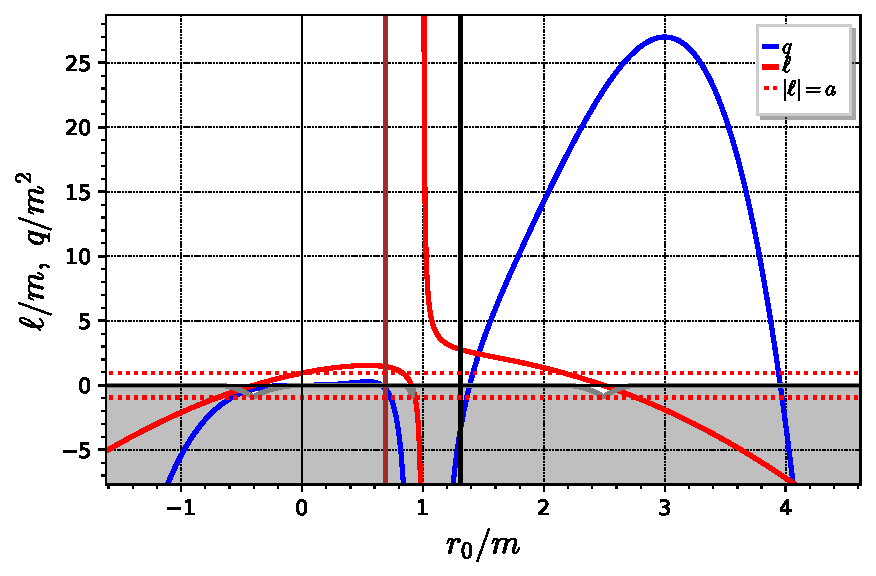
\includegraphics[width=0.49\textwidth]{gik_spher_orb_exist.pdf}\
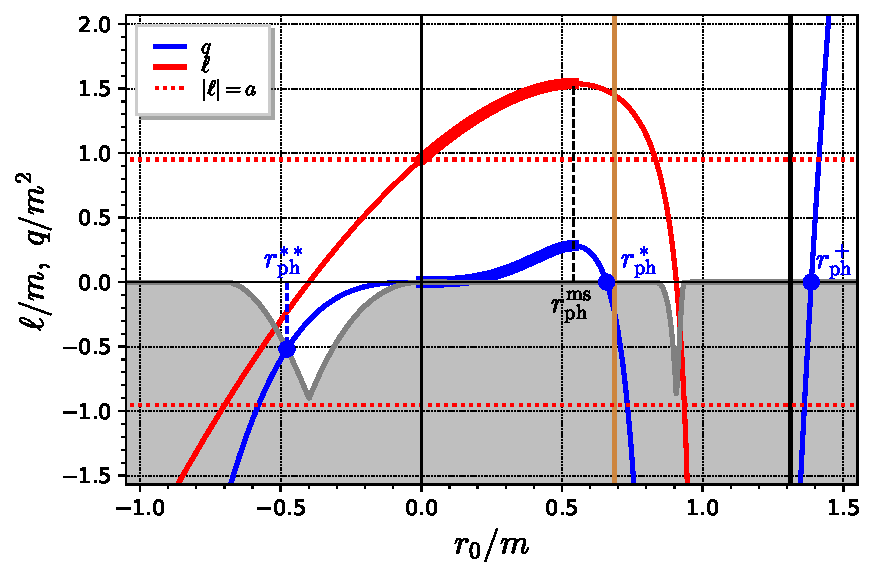
\includegraphics[width=0.49\textwidth]{gik_spher_orb_exist_zoom.pdf}}
\caption[]{\label{f:gik:spher_orb_exist} \footnotesize
Functions $\ell(r_0)$ (in red) and $q(r_0)$ (in blue) giving the reduced angular momentum
and reduced Carter constant of a spherical photon orbit of radius $r_0$,
according to Eqs.~(\ref{e:gik:spher_ell_r0}) and (\ref{e:gik:spher_q_r0})
and for $a=0.95\, m$. The right figure is a zoom on the part
$-m\leq r_0 \leq 3m/2$. The thick vertical lines
mark the two horizons: $\Hor$ (black) and $\Hor_{\rm in}$ (light brown).
The horizontal dotted lines mark the boundary of the region $|\ell|<a$,
where $q$ can take negative values. Values of $q$ in the grey zone
are unphysical, i.e. do not fulfil the conditions (\ref{e:gik:q_constraints}),
so that only values of $r_0$ for which the blue curve lies
above the grey zone correspond to spherical photon orbits. This occurs
for $r_{\rm ph}^{**} \leq r_0 \leq r_{\rm ph}^*$ and $r_{\rm ph}^+ \leq r_0 \leq r_{\rm ph}^-$.
\textsl{[Figure generated by the notebook \ref{s:sam:Kerr_spher_photon_existence}]}
}
\end{figure}

Equations~(\ref{e:gik:spher_ell_r0}) and (\ref{e:gik:spher_q_r0}) provide
the general solution to the system $\mathcal{R}(r_0) = 0$ and $\mathcal{R}'(r_0) = 0$
[Eq.~(\ref{e:gik:R_Rp_r0_zero})], but not all
of them correspond to spherical photon orbits. Indeed, we do not expect
spherical photon orbits to exist for any value of $r_0$, in particular
for $|r_0|\gg m$. Actually, not all values of $q$ given by Eq.~(\ref{e:gik:spher_q_r0})
are permitted, but only those that fulfill the constraints established in
Sec.~\ref{s:gik:th_motion}, namely
\begin{subequations}
\label{e:gik:q_constraints}
\begin{align}
    & q \geq 0 \quad \mbox{if}\  |\ell| \geq a \label{e:gik:q_constraints_1}\\
    & q \geq - \left( a - |\ell| \right) ^2  \quad \mbox{if}\  |\ell| < a . \label{e:gik:q_constraints_2}
\end{align}
\end{subequations}
The solutions $\ell$ and $q$ given by Eqs.~(\ref{e:gik:spher_ell_r0})-(\ref{e:gik:spher_q_r0})
are plotted as functions of $r_0$ for $a=0.95\, m$
in Fig.~\ref{f:gik:spher_orb_exist}, where the
region excluded by (\ref{e:gik:q_constraints}) is colored in grey. Consequently
spherical photon orbits exist only for values of $r_0$ for which the $q$ curve
(in blue) lies above the grey region. We see that this occurs in two intervals:
\be \label{e:gik:spher_orb_range}
    \encadre{ r_0 \in [r_{\rm ph}^{**}, r_{\rm ph}^*] }
    \qand
    \encadre{ r_0 \in [r_{\rm ph}^+, r_{\rm ph}^-] },
\ee
where $r_{\rm ph}^*$, $r_{\rm ph}^+$ and $r_{\rm ph}^-$ are the three (ordered) roots
distinct from $0$ of the equation $q(r_0) = 0$ (boundary for
condition (\ref{e:gik:q_constraints_1})) and $r_{\rm ph}^{**}$ is the unique
root of the equation $q(r_0) = - \left( a - |\ell(r_0)| \right) ^2$ when
$|\ell(r_0)|  < a$ (boundary for condition (\ref{e:gik:q_constraints_2})).
The above reasoning is based on Fig.~\ref{f:gik:spher_orb_exist}, which has
been drawn for $a=0.95\, m$; however the conclusions (\ref{e:gik:spher_orb_range})
hold for any value of $a$ (see the notebook~\ref{s:sam:Kerr_spher_photon_existence}
for figures with $a=0.5\, m$ or $a=0.998\, m$).

Given expression (\ref{e:gik:spher_q_r0}) for $q$, we see that
$r_{\rm ph}^*$, $r_{\rm ph}^+$ and $r_{\rm ph}^-$
are the three roots of the cubic equation
\be
r_0(r_0 - 3m)^2 - 4 a^2 m  = 0 .
\ee
We can solve this equation by bringing it to a depressed form in order
to use Viète's formulas (\ref{e:gis:Viete}). However, we may rely on an
already solved equation by noticing the following equivalences:
\begin{eqnarray}
r_0(r_0 - 3m)^2 - 4 a^2 m  = 0  & \iff & r_0 \geq 0 \ \ \mbox{and} \ \
            \sqrt{r_0} | r_0 - 3 m | = 2 a\sqrt{m} \nonumber \\
& \iff &  r_0 \geq 0 \ \ \mbox{and} \ \
    \sqrt{r_0} (r_0 - 3 m ) \pm 2 a \sqrt{m} = 0 \nonumber \\
& \iff &  r_0 \geq 0 \ \ \mbox{and} \ \
    r_0^{3/2} - 3 m r_0^{1/2} \pm 2 a \sqrt{m} = 0 , \nonumber
\end{eqnarray}
where $\pm$ is $+$ for $r_0 \leq 3 m$ and $-$ for $r_0 \geq 3m$.
We recognize the function of $r_0$ which appears in the left-hand side
of Eq.~(\ref{e:gek:cubic_sqrt_r0}). As shown in Sec.~\ref{s:gek:existence_circ_orb},
there are three real roots,
$r_{\rm ph}^*$, $r_{\rm ph}^+$ and $r_{\rm ph}^-$, with
$r_{\rm ph}^*, r_{\rm ph}^+\leq 3m$ ($\pm = +$)
and $r_{\rm ph}^- \geq 3m$ ($\pm = -$). They are given by Eqs.~(\ref{e:gek:def_r_star})
and (\ref{e:gek:def_r_min_pm}):
\be \label{e:gik:rph_s}
   \encadre{ r_{\rm ph}^* := 4m\cos^2 \left[ \frac{1}{3} \arccos\left(-\frac{a}{m} \right)  + \frac{4\pi}{3} \right] } .
\ee
\be \label{e:gik:rph_pm}
   \encadre{ r_{\rm ph}^\pm := 4m\cos^2 \left[ \frac{1}{3} \arccos\left( \mp \frac{a}{m} \right) \right] }
\ee
As for $r_{\rm ph}^{**}$, since $q(r_0) = - (a - |\ell(r_0)|)^2$ with
$|\ell(r_0)|  < a$ occurs in a region where $\ell(r_0) < 0$ (cf. Fig.~\ref{f:gik:spher_orb_exist}),
we get that $r_{\rm ph}^{**}$ is a solution of the equation
$q(r_0) = - (a + \ell(r_0))^2$. Given expressions (\ref{e:gik:spher_ell_r0}) and (\ref{e:gik:spher_q_r0})
for respectively $\ell(r_0)$ and $q(r_0)$, we get that $r_{\rm ph}^{**}$ is a root of the cubic
equation
\be \label{e:gik:cubic_rph_ss}
    2 r_0^3 - 3 m r_0^2 + a^2 m = 0 .
\ee
By the change of variable $r_0 =: x + m/2$, we turn this equation into a depressed one:
\[
    x^3  - \frac{3}{4} m^2 x + \frac{m}{2} \left(a^2 - \frac{m^2}{2} \right) = 0 ,
\]
i.e. $x^3 + px + q = 0$, with $p:= -3m^2/4$ and $q:=(m/2)(a^2 - m^2/2)$.
The discrimant is $-(4 p^3 + 27 q^2) = 27 a^2 m^2 (m^2 - a^2)/4 \geq 0$. The three roots
$(x_k)_{k\in\{0,1,2\}}$ are then all real and are given by Viète's formula (\ref{e:gis:Viete}).
Only the root $x_1$ leads to a negative value of $r_0$, which is the value we
are looking for (cf. Fig.~\ref{f:gik:spher_orb_exist}). Viète's formula (\ref{e:gis:Viete})
with $k=1$ yields
\[
    x_1 = m \cos\left[ \frac{1}{3} \arccos\left(1 - 2 \frac{a^2}{m^2} \right) + \frac{2\pi}{3} \right]
        = m \cos\left[ \frac{2}{3} \arcsin\left(\frac{a}{m}\right) + \frac{2\pi}{3} \right] ,
\]
from which we obtain
\be \label{e:gik:rph_ss}
   \encadre{ r_{\rm ph}^{**} = \frac{m}{2} + m \cos\left[ \frac{2}{3} \arcsin\left(\frac{a}{m}\right) + \frac{2\pi}{3} \right] } .
\ee

\begin{figure}
\centerline{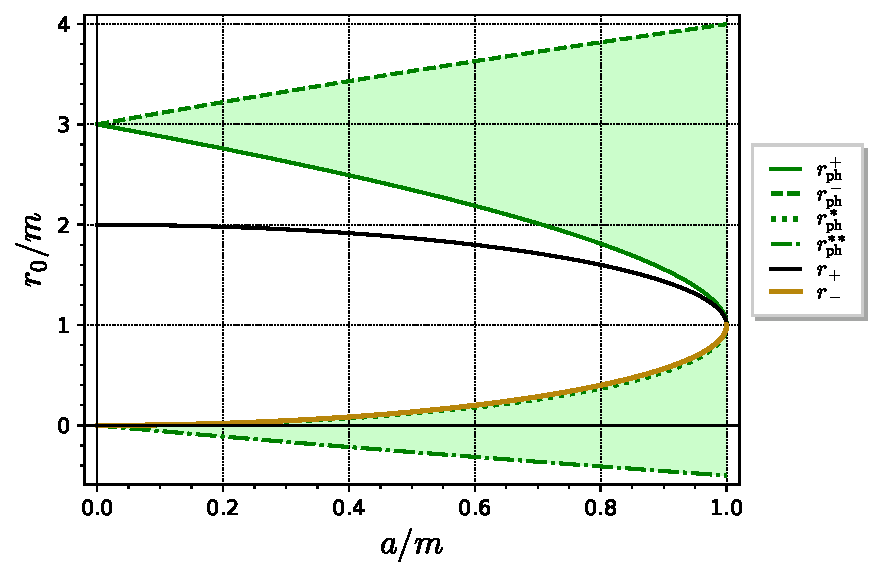
\includegraphics[width=0.7\textwidth]{gik_spher_orb_range.pdf}}
\caption[]{\label{f:gik:spher_orb_range} \footnotesize
Domain of existence of spherical photon orbits in the $(a, r_0)$ plane
(in green). The boundaries of the domain are the radii
$r_{\rm ph}^{**}$, $r_{\rm ph}^*$, $r_{\rm ph}^+$ and $r_{\rm ph}^-$
given by Eqs.~(\ref{e:gik:rph_ss}), (\ref{e:gik:rph_s}) and (\ref{e:gik:rph_pm}).
The black curve indicates the black hole horizon $\Hor$ and the light brown one
the inner horizon $\Hor_{\rm in}$.
\textsl{[Figure generated by the notebook \ref{s:sam:Kerr_spher_photon_existence}]}
}
\end{figure}

The four critical radii $r_{\rm ph}^{**}$, $r_{\rm ph}^*$, $r_{\rm ph}^+$ and $r_{\rm ph}^-$
are plotted in terms of $a$ in Fig.~\ref{f:gik:spher_orb_range}. We notice that
\be
  \encadre{  - \frac{m}{2} \leq r_{\rm ph}^{**} \leq 0 \leq r_{\rm ph}^* \leq r_- \leq m \leq r_+ \leq r_{\rm ph}^+
    \leq 3 m \leq r_{\rm ph}^- \leq 4 m },
\ee
with the limits (\ref{e:gek:lim_rph_pm}) and (\ref{e:gek:lim_rph_s}). In addition,
\be
    \lim_{a\to 0} r_{\rm ph}^{**} = 0 \qand
    \lim_{a\to m} r_{\rm ph}^{**} = - \frac{m}{2} .
\ee
As already stressed in Sec.~\ref{s:gek:existence_circ_orb}, $r_{\rm ph}^*$ is lower than, but very close to,
the inner horizon radius $r_{-}$, with  $\max (r_- - r_{\rm ph}^*) \simeq 0.032 \, m$,
achieved for $a\simeq 0.9 \, m$.
In view of the above inequalities and the ranges (\ref{e:gik:spher_orb_range}), we conclude that
\begin{greybox}
Spherical photon orbits exist in two regions of Kerr spacetime:
\begin{itemize}
\item orbits with $r_0\in [r_{\rm ph}^{**}, r_{\rm ph}^*]$ are located in $\M_{\rm III}$;
we shall call them the \defin{inner spherical photon orbits}\index{inner!spherical photon orbit}\index{spherical!photon orbit!inner --}\index{photon!orbit!inner spherical --};
\item orbits with $r_0 \in [r_{\rm ph}^+, r_{\rm ph}^-]$ are located in $\M_{\rm I}$;
we shall call them the \defin{outer spherical photon orbits}\index{outer!spherical photon orbit}\index{spherical!photon orbit!outer --}\index{photon!orbit!outer spherical --}.
\end{itemize}
\end{greybox}

\begin{figure}
\centerline{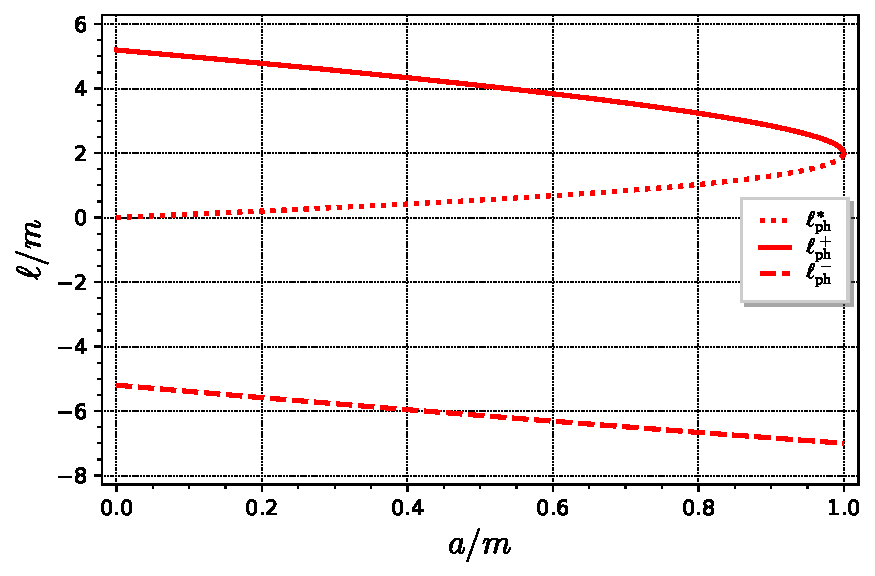
\includegraphics[width=0.6\textwidth]{gik_ell_circ_equat.pdf}}
\caption[]{\label{f:gik:ell_circ_equat} \footnotesize
Reduced angular momentum $\ell$ of the three circular photon orbits in the
equatorial plane, as a function of the Kerr spin parameter $a$.
\textsl{[Figure generated by the notebook \ref{s:sam:Kerr_spher_photon_existence}]}
}
\end{figure}


The spherical orbits with $r_0 = r_{\rm ph}^*$, $r_{\rm ph}^+$ and $r_{\rm ph}^-$ have $q=0$
and $|\ell| > a$. According to the results of Sec.~\ref{s:gik:th_motion}, they
necessary lie in the equatorial plane $\th=\pi/2$. They are thus \emph{circular}
orbits. According to expression~(\ref{e:gik:spher_q_r0}) for $q$, they are the
only ones in the equatorial plane, because the only other root of $q(r_0)=0$ is $r_0=0$
(see also Fig.~\ref{f:gik:spher_orb_exist}),
which would correspond to the ring singularity.
Let us denote by $\ell_{\rm ph}^*$, $\ell_{\rm ph}^+$ and $\ell_{\rm ph}^-$
the reduced angular momentum $\ell$ of respectively the
circular photon orbit at $r_{\rm ph}^*$, $r_{\rm ph}^+$ and $r_{\rm ph}^-$.
These values of $\ell$ are deduced from Eq.~(\ref{e:gik:spher_ell_r0}) and
are plotted in terms of $a$ in Fig.~\ref{f:gik:ell_circ_equat}.
We have $\ell_{\rm ph}^*>0$, $\ell_{\rm ph}^+>0$ and $\ell_{\rm ph}^-<0$.
Moreover,
\be
    \lim_{a\to 0} \ell_{\rm ph}^+ =  \lim_{a\to 0} \left| \ell_{\rm ph}^- \right|
    = 3\sqrt{3} m \simeq 5.196\, m ,
\ee
in agreement with the Schwarzschild result (\ref{e:ges:b_crit}), while
\be
    \lim_{a\to m} \ell_{\rm ph}^+ =  \lim_{a\to m} \ell_{\rm ph}^* = 2 m,
\ee
in agreement with Eq.~(\ref{e:gik:spher_orb_r0_eq_m}), since
$\lim_{a\to m} r_{\rm ph}^+ = \lim_{a\to m} r_{\rm ph}^* = m$.

The spherical orbits with $r_0 = r_{\rm ph}^{**}$ have
$q < 0$, i.e. are vortical geodesics. Moreover, they fulfill $q=q_{\rm min}=-(a - |\ell|)^2$.
According to the results of Sec.~\ref{s:gik:th_motion}, this corresponds to two orbits at
a fixed value of $\th$, which are symmetrical with respect to the equatorial plane.
They lie at $\th = \th_{\rm ph}^{**}$ (Northern hemisphere) and
$\th = \pi - \th_{\rm ph}^{**}$ (Southern hemisphere), where
$\th_{\rm ph}^{**}$ is given by Eq.~(\ref{e:gik:th_s_ell_over_a}), using
for $\ell$ the value (\ref{e:gik:spher_ell_r0}) with $r_0 = r_{\rm ph}^{**}$.
Since $3 m (r_{\rm ph}^{**})^2 = 2 (r_{\rm ph}^{**})^3 + a^2 m$ by virtue of
Eq.~(\ref{e:gik:cubic_rph_ss}), some simplification occurs and we get
\be
    \th_{\rm ph}^{**} =  \arcsin\sqrt{\frac{|r_{\rm ph}^{**}|}{m - r_{\rm ph}^{**}}
    \left( 1 - \frac{(r_{\rm ph}^{**})^2}{a^2} \right)} .
\ee
$\th_{\rm ph}^{**}$ is an increasing function of $a/m$, plotted in Fig.~\ref{f:gik:theta_ss}.
We have $\lim_{a\to 0} \th_{\rm ph}^{**} = 0$ (the rotation axis) and
$\lim_{a\to m} \th_{\rm ph}^{**} = \pi/6$.
Since they occur at a fixed value of $\th$, the two vortical spherical photon orbits
are actually circular. Their reduced angular momentum and Carter constant,
denoted by $\ell_{\rm ph}^{**}$ and
$q_{\rm ph}^{**}$ respectively,
are shown in terms of $a$ in Fig.~\ref{f:gik:ell_q_rss}.
They tend to zero as $a\to 0$ and obey
\be
    \lim_{a\to m} \ell_{\rm ph}^{**} = - \frac{m}{4} \qand
    \lim_{a\to m} q_{\rm ph}^{**} = - \frac{9}{16} m^2 .
\ee

\begin{figure}
\centerline{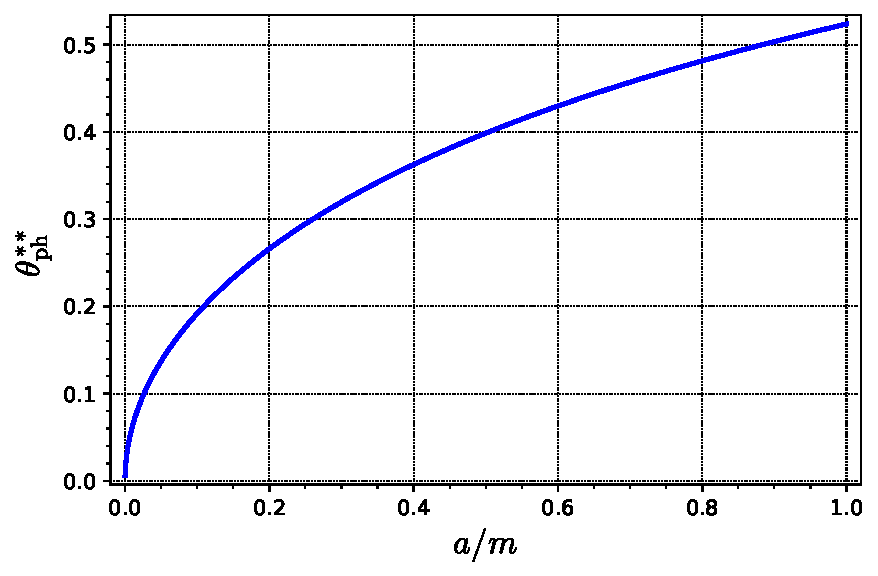
\includegraphics[width=0.6\textwidth]{gik_theta_ss.pdf}}
\caption[]{\label{f:gik:theta_ss} \footnotesize
Angle $\th$ of the Northern vortical circular photon orbit at $r = r_{\rm ph}^{**}$ as a
function of Kerr spin parameter $a$.
\textsl{[Figure generated by the notebook \ref{s:sam:Kerr_spher_photon_existence}]}
}
\end{figure}

\begin{figure}
\centerline{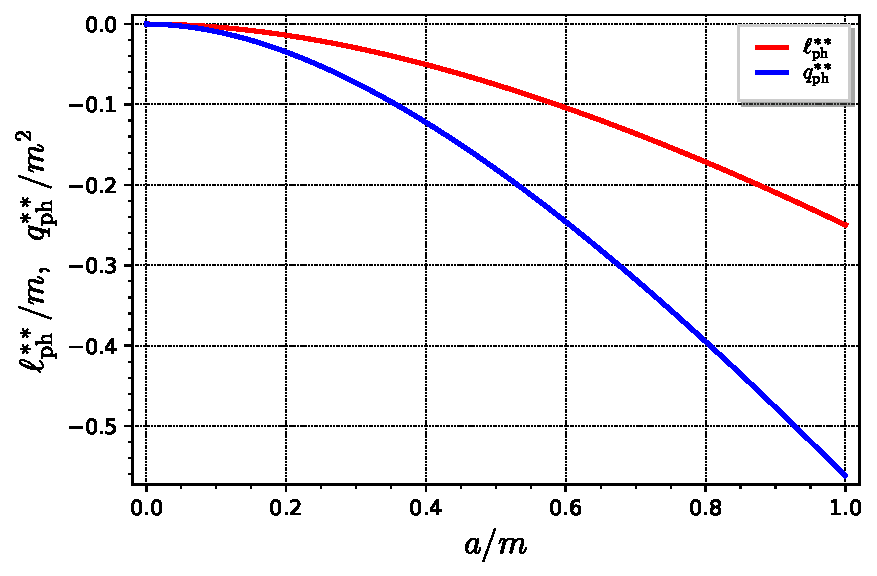
\includegraphics[width=0.6\textwidth]{gik_ell_q_rss.pdf}}
\caption[]{\label{f:gik:ell_q_rss} \footnotesize
Reduced angular momentum $\ell_{\rm ph}^{**}$ and reduced Carter constant
$q_{\rm ph}^{**}$ of the two vortical circular photon orbits
at $r = r_{\rm ph}^{**}$, as
functions of Kerr spin parameter $a$.
\textsl{[Figure generated by the notebook \ref{s:sam:Kerr_spher_photon_existence}]}
}
\end{figure}

We may summarize the above results by
\begin{greybox}
The geodesics at the boundaries of the domain of
existence of spherical photon orbits [Eq.~(\ref{e:gik:spher_orb_range})] are circular orbits, having a fixed value of $(r,\th)$:
\begin{itemize}
\item the orbit at $(r,\th)=(r_{\rm ph}^{**},\th_{\rm ph}^{**})$ is called
the \defin{Northern vortical circular photon orbit}\index{vortical!circular photon orbit}\index{circular!photon orbit!vortical --};
\item the orbit at $(r,\th)=(r_{\rm ph}^{**},\pi - \th_{\rm ph}^{**})$ is called
the \defin{Southern vortical circular photon orbit};
\item the orbit at $(r,\th)=(r_{\rm ph}^*,\pi/2)$ is called the \defin{equatorial inner circular photon orbit}\index{equatorial!circular photon orbit}\index{inner!circular!photon orbit};
\item the orbit at $(r,\th)=(r_{\rm ph}^+,\pi/2)$ is called the \defin{prograde outer circular photon orbit}\index{prograde!outer circular!photon orbit};
\item the orbit at $(r,\th)=(r_{\rm ph}^-,\pi/2)$ is called the \defin{retrograde outer circular photon orbit}\index{retrograde!outer circular!photon orbit};
\end{itemize}
\end{greybox}



%This is not surprising since $q=0$ implies equatorial orbits, i.e. necessarily
%circular ones.

\subsection{Photon region}

\section{Images}

















